\chapter{Player behavior modeling in~\glsdesc{pirg}}\label{ch:modeling}

%ANDY This chapter contains parts that are general enough to become part of the introduction, and frame the whole thesis, other parts that are quite specific to a paper (and it is worth to state explicitly that they have been published), other parts that could be related to other parts of the thesis. I have put comments. Let's try to have something more similar to a chapter of a thesis, integrated in the thesis flow, than just a paper put here out of the blue.

In this chapter we present our approach for player modeling in~\gls{pirg}, beginning from the activity recognition system described in the previous chapter.

\section{A simple activity model}
Having identified an activity system, we aimed at the definition of an approach to model user behavior that could account for the combination of the player physical effort and interaction level. The proposed model is based on the human activity recognition (see chapter~\ref{ch:activity}) and a description of interaction (proximity and body contraction index) relative to the robot co-player. %ANDY If you have described separately the activity recognition model based on the accelerometer, a separate chapter has to be dedicated also to the lasers or whatever you would like to consider for the other parameters.  All these sources are functional toprovide data for the activity model (if you like you may have all the contributions in the same chapter).

\section{Relational Activity Model}\label{theModel}

As in~\cite{etheredge_generic_2013}, we defined as behavior a sequence of discrete time-bounded actions performed by the player. Since we are dealing with a physically interactive scenario, these time-bounded actions have strong relation with the amount of physical activity spent, hereby considered as the human ``activity effort''. The relationship with the robot, on the other hand, is considered the ``relative interaction''. 

In the proposed model, the two dimensions (activity and interaction) are combined into a simple overall scoring system capable of describing quantitatively the player's active participation in the~\gls{pirg}. The proposed model is detailed in the next.

\subsubsection{Activity}\label{activity}

Equation~\ref{eq:activity_eq} is used to compute the general amount of activity $\alpha(m)$, given the classification of primitive motions from chapter~\ref{ch:activity}:

\begin{equation}
	\alpha(m)=\sum_{i \in \mathcal{A}} \omega_{i}\varphi_i(m);\qquad m \in \mathcal{M}
	\label{eq:activity_eq}
\end{equation}
, where $\mathcal{A}$ stands for the set of activities \{``running'', ``locally moving'', ``walking/dodging''\}; $\omega$ stands for the activity weight; $\varphi$ for the stochastic prediction value for the motion primitive $m$.

We consider equation~\ref{eq:activity_eq} as a measure of the ``effort'' of the player. The weight $\omega$ states how much each physical activity contributes to the overall quantification and is a hyper-parameter.

\subsection{Interaction}\label{Interaction}
In order to model the interaction we take into account the spatial relationship between the player and the robot defined as ``proximity'' and a measure of body contraction named ``contraction index'' (CI).

Proximity is a measure defined in the interval [0, 1], computed from the data provided by the Microsoft Kinect\textsuperscript{\textregistered}, normalized given the sensor specifications (see section~\ref{sec:kinectsec}). CI is also in [0 , 1] and it is calculated using a technique related to the bounding region, i.e., the minimum rectangle surrounding the body: the algorithm compares the area covered by this rectangle with the area currently covered by the player's silhouette~\cite{castellano_recognising_2007}.

A high CI is associated with an intense interaction because a wide openness of the body is interpreted as a higher focus level of the player w.r.t the robot and to the game; for this reason it will boost the final outcome. Low CI, in turn, is interpreted as a lack of focus or, in general, limited motivation of the player, which penalizes the interaction. %ANDY Not providing data and analysis to support this makes this assumption quite weak

\subsection{Combined model}\label{sec:engagement}
The model to describe the player's relational activity is a combination of the activity level and the degree of interaction, named $\epsilon$; it summarizes the player physical activity during the game, weighted by his interaction with the robotic opponent as follows: 
\begin{equation}
\label{enagementeq}
\epsilon=\kappa\alpha(m),
\end{equation}

where $\kappa= (1-\rho)$ and uses the degree of interaction $\rho$ so that when the output of the fuzzy %ANDY fuzzy? Never mentioned till now
 system is zero (meaning no interaction) the activity level is only the activity $\alpha$. In other cases, $\kappa$ is the multiplying factor that boosts the importance of the activity by putting it in relation with the amount of interaction.  %ANDY actually, if k ranges in [0 1] and multplies alpha, it will reduce alpha...
Notice, however, that $\rho$ is an overall degree of interaction, i.e., the combination of CI and proximity. The exact procedure for the combination of the interaction signals is not bound to a specific method. In this work, we have used a fuzzy logic system to obtain the desired combination, described in a linguistic way. In principle, the combination of the signals depends on the specifics of the~\gls{pirg} environment.
%ANDY I donot remember what mentioned above and seems to me quite confused. Let's talk about it.


\subsection{Evaluation}\label{sec:simple_evalution}
\subsubsection{Data elaboration}
We considered 29 matches involving 15 male participants of different ages. The age distribution consisted of children (7-10) and adults (26-40). This sample matches the typical user distribution for this kind of games, and arose in uncontrolled way from the presentation of the game to general public (including differently aged people, males and females) in an exhibition context. The variety of behaviors collected in these trials was high and supported our hypothesis about the need of an adapting robot. In these matches, the robot was remotely driven by a human operator. Matches had a minimum time duration of about 40 secs and a maximum of about 1 minute and 10 secs. 

The collected data are the acceleration values along x, y, and z axis with a sampling frequency of 50Hz, which is five times larger than the frequency considered to be sufficient for detecting daily activities from accelerometer data (10Hz)~\cite{kikhia_analyzing_2014}. %ANDY This was already mentioned in another section

In terms of dataset support, 34$\%$ of the motion primitives correspond to locally moving (LM); 25$\%$ to walking/dodging (WD) and 41$\%$ running (R). %ANDY This was already mentioned in another section

We use a sliding window half a second long, with 10\% overlap, for the STD graph generation. In our experiments, the produced spikes in variance have a huge discriminative power w.r.t. activities demanding sudden changes in behavior, e. g., a ``running'' motion. We also used a positive half sine wave as windowing function in order to soften the transition between windows. As mentioned, the ``inactive'' type is not considered in the recognition task since it is directly classified by the inactive threshold line. 
%ANDY This resembles, but adds something what was already mentioned in another section    

\subsubsection{Model results}
The model output for two different players can be seen in figure~\ref{fig:modelOutput}. In figure~\ref{fun}, the player is perceived as more active than the one in fig.~\ref{nofun}. The ratio between activity and inactivity exposed by the output matches the observed data and empirically confirms the model viability.

\begin{figure}[h!]
    \centering 
	\begin{subfigure}[H]{0.3\textwidth}
		\centering      
		\includegraphics[width=\columnwidth]{images/04-activity/combined.png}
		\caption{}
		\label{fig:fun}
	\end{subfigure}
	~
	\begin{subfigure}[H]{0.3\textwidth}
		\centering      
      	\includegraphics[width=\columnwidth]{images/04-activity/combined_less.png}
      	\caption{}
      	\label{fig:nofun}
     \end{subfigure}
      \caption{a) Model results for a single match that lasted 45 secs. b) Model output for a less active player. The graph refers to 30 initial secs of activity.}		
      \label{fig:modelOutput}
\end{figure}

The model quantitatively describe, in a simple way, the player's relational activity by the combination of the amount of physical activity and interaction relative to the robot. This can be used as a metric expected to enable the robot to take into account the player's attitude in order to adapt its own activity to match it. Using this model, for instance, an active player could be viewed as one having a larger cumulative sum of $\epsilon$ values up to a point in time.

However, this model is limited in several ways, %ANDY I cannot evaluate it since I cannot understand it
one of which is the manual definition of weights for the activities ($\omega$). Manually selecting these weights becomes difficult as the number of activities grows. We have then worked on a definition of a more robust player model relying on latent representation. This is describe next.

\section{Latent player modeling}

\subsection{Introduction} %ANDY see comment above
We attempted to mitigate the limitations in the previous model by first mapping the stream of data to an image representation, namely a Gramian Angular Field (GAF)~\cite{wang_imaging_2015}, which is subsequently processed by a simple autoencoder~\cite{goodfellow_deep_2016} architecture for unsupervised feature extraction. %ANDY Why would this limit the issues of the previous simple model?

After the definition of a dictionary of primitives on the feature space, we apply latent Dirichlet allocation (\gls{lda}~\cite{blei_latent_2003}), a generative model mostly used for document retrieval and classification, to uncover coherent groups of motion patterns that can be used to categorize players.

Our decision to use \gls{lda} takes inspiration from recent approaches where each game session is represented as a ``document'', and chunks of generated stream data are encoded into discrete ``words''~\cite{smith_mining_2016}. This arrangement is based on the assumption that different players generate different streams of input words, thus different documents, depending on their own motivation or play style. 

The possibility to apply \gls{lda} to this problem is further reinforced by noticing the apparent difficulty in objectively separating types of motion patterns, since a player in his/her playing activity may show one or more different motion styles. More explicitly, a player may, for instance, become bored or frustrated with the game and consequently show a low motion profile w.r.t. the one that the same player might have shown in other moments during the same game session, for instance, when he/she was excited about it. Here, we consider that a high motion profile, i.e., high turbulence in acceleration signal, is typical for a highly motivated player, since by common sense %ANDY this should not be assessed by common sense, but by data
, a non-motivated player {tends} to stay relatively still, or to show a very low acceleration signal.

The claim that motion style conveys engagement or even emotion~\cite{aristidou_emotion_2015,shafir_emotion_2016,tsachor_somatic_2017} types has been supported by several papers. As an example, systematic approaches for describing movement, such as~\gls{lma}~\cite{laban_language_1974}, are often used to derive low-dimensional representation of movement, facilitating affective motion modeling~\cite{burton_laban_2016}. This same type of analysis has been applied when investigating motor elements that characterize movements whose execution enhances basic emotions, such as: anger, fear, happiness and sadness~\cite{shafir_emotion_2016}. In game situations, despite the limited capacity for entertainment detection and modeling in Exergames, \gls{lma} had been reported as useful in fostering emotion recognition in states like: concentration, meditation, excitement and frustration~\cite{zacharatos_emotion_2013}.

Here, we hypothesize that, on average, a player will display his/her game-intrinsic motion style and convey some information about his/her interest in/motivation to play. Discovering which coherent groups of motion style exist in a dataset allows us to estimate to what extent an unknown player relates in terms of his/her own motion profile to known groups. This may ultimately support the design of \gls{pirg}s able to adapt in order to offer a better play experience.

Following this, in this manuscript, a player representation is addressed as how much of each discovered motion types to which we are confident to say a given player is mostly related. %ANDY To be rephrased, it is so involute that I can hardly understand, and I do not touch it
We call this representation a {mixture proportion of motion types} (similar to topics in the LDA perspective). 

In summary, we expect to see that similar player-generated data are grouped together in a coherent collection, enabling to distinguish among motion types. The results obtained are validated with human supervision, %ANDY Why <- should be supported by this -> ?
suggesting the applicability of our method to future mechanisms for designing auto-adapting \gls{pirg}s agents.

\subsection{Mathematical Preliminaries}

This section presents the basic concepts and principles of the Gramian angular field, autoencoders and latent Dirichlet allocation, our targeted probabilistic graphical model. %ANDY Again, this would call for distributing the state of art section.

\subsubsection{Gramian Angular Field Images}

The results obtained in this work rely on the transformation of the time series data generated by the player motion into images that can then be processed and understood in terms of emergent patterns that can, in turn, be discovered by state-of-the-art machine learning algorithms. The type of image we have chosen is Gramian Angular Summation/Difference Field (GASF/GADF). Such images had been proposed in the field of time series classification~\cite{wang_imaging_2015}, where the authors evaluated the efficacy of representing time series in a polar coordinate system instead of the typical Cartesian coordinates. For a deep understanding of the method, we suggest reading the original paper, where the authors did not only present the idea of GASF/GADF, but also reported experimental results comparing them with other time series imagery techniques. Here, we present an overview of the technique in order to familiarize the reader with such a method and to point out its role in our proposal.

In general, in order to obtain a GASF/GADF representation for a time series $\mathcal{X}=\{x_{1}, x_{2}, ... x_{n}\}$ of size $n \in \mathbb{N}_{>0}$, rescaling is first performed in order to put the time series in the interval $[\,-1,1] \,$ or $[\,0,1]\,$. The second step is to represent the rescaled time series $\widetilde{\mathcal{X}}$ in polar coordinates, where each sample value is now mapped into the angular cosine and the time stamp information is represented as the radius. 
The formula for this step is as follows:

\begin{equation}
\begin{dcases}
  \phi = \arccos(\widetilde{x}_{i}) \quad -1 \leq \widetilde{x}_{i} \leq 1, \widetilde{x}_{i} \in \widetilde{\mathcal{X}} \\
  r = \frac{t_{i}}{N} \quad \quad t_{i} \in \mathbb{N}_{>0},
\end{dcases}
\label{equation:GAF}
\end{equation} 
where $t_{i}$ is the time stamp and $N$ plays the role of a normalizer for the span of the polar coordinate system. Some properties of this transformation are known:

\begin{itemize}[leftmargin=*,labelsep=5.8mm]
\item {Property \#1}: The encoding map of Equation~(\ref{equation:GAF}) is bijective as $\cos(\phi)$ is monotonic when $\phi \in [\,0,\pi]\,$. Given a time series, the proposed map produces a unique result in the polar coordinate system together with a unique inverse map. 
\item {Property \#2}: As opposed to Cartesian coordinates, polar coordinates preserve absolute temporal~relations.
\item {Property \#3}: Rescaled data in different intervals have different angular bounds. That is, $[\,0,1]\,$ corresponds to the cosine function in $[\,0,\frac{\pi}{2}]\,$, while cosine values in the interval $[\,-1,1]\,$ fall into the angular bounds $[\,0,\pi]\,$. These intervals are known to produce different information granularity in the Gramian angular field, especially for classification tasks~\cite{wang_imaging_2015}.
\end{itemize}

The third step in completing the transformation is to exploit the angular perspective by considering the trigonometric sum/difference between each point. This allows for the identification of the temporal correlation within different time intervals. The two types of GAFs, namely GASF and GADF, are obtained as follows:

\begin{equation}
\begin{aligned}
GASF &= [\,\cos(\phi_{i} + \phi{j}]\, \\
	 &= \widetilde{\mathcal{X}}' \cdot \widetilde{\mathcal{X}} - \sqrt{I-\widetilde{\mathcal{X}}^2}' \cdot \sqrt{I-\widetilde{\mathcal{X}}^2}
\end{aligned}
\end{equation}
\\
\begin{equation}
\begin{aligned}
GADF &= [\,\sin(\phi_{i} + \phi{j}]\, \\
	 &= \sqrt{I-\widetilde{\mathcal{X}}^2}' \cdot \widetilde{\mathcal{X}} - \widetilde{\mathcal{X}}' \cdot \sqrt{I-\widetilde{\mathcal{X}}^2}\\
\end{aligned}
\end{equation}

$I$ is the unit row vector. After translating the time series from the Cartesian to polar coordinate system, each time step in it is taken as a 1D metric space. By defining the inner product as $<x,y> = x \cdot y - \sqrt{1-x^2} \cdot \sqrt{1-y^2}$ and $<x,y> = \sqrt{1-x^2} \cdot y - x \cdot \sqrt{1-y^2}$,
respectively, the GAFs become {quasi-Gramian} matrices, since the defined $<x,y>$ do not satisfy the property of linearity in inner-product space.

Still, according to~\cite{wang_imaging_2015}, the GAFs have several advantages:

\begin{itemize}[leftmargin=*,labelsep=5.8mm]
\item {Advantage \#1}: They provide a way to preserve temporal information. The temporal correlation is present because $G_{(i,j||i-j|=k)}$ represents the relative correlation by the superposition/difference of directions with respect to time interval $k$. The main diagonal $G_{i,i}$ is the special case when $k = 0$, which contains the original value/angular information. 
\item {Advantage \#2:} From the main diagonal, it is possible to reconstruct the time series back into the original Cartesian space. This is useful especially in a classification task, where we can convert the time series back to numerical Cartesian space from the high level features learned by, for instance, a deep neural network.
\end{itemize}

However, the size of the Gramian matrix $G$ is $n \times n$, for $n$ being the length of the raw time series. The authors propose a solution for this issue by attempting to reduce the size of the produced GAFs using, for instance, Piecewise Aggregation Approximation (PAA)~\cite{keogh_scaling_2000} to smooth the time series while preserving the trends. An example of the conversion from time series to GASF image is shown in Figure~\ref{figure:gasf_example}.

\begin{figure} [H]
\centering
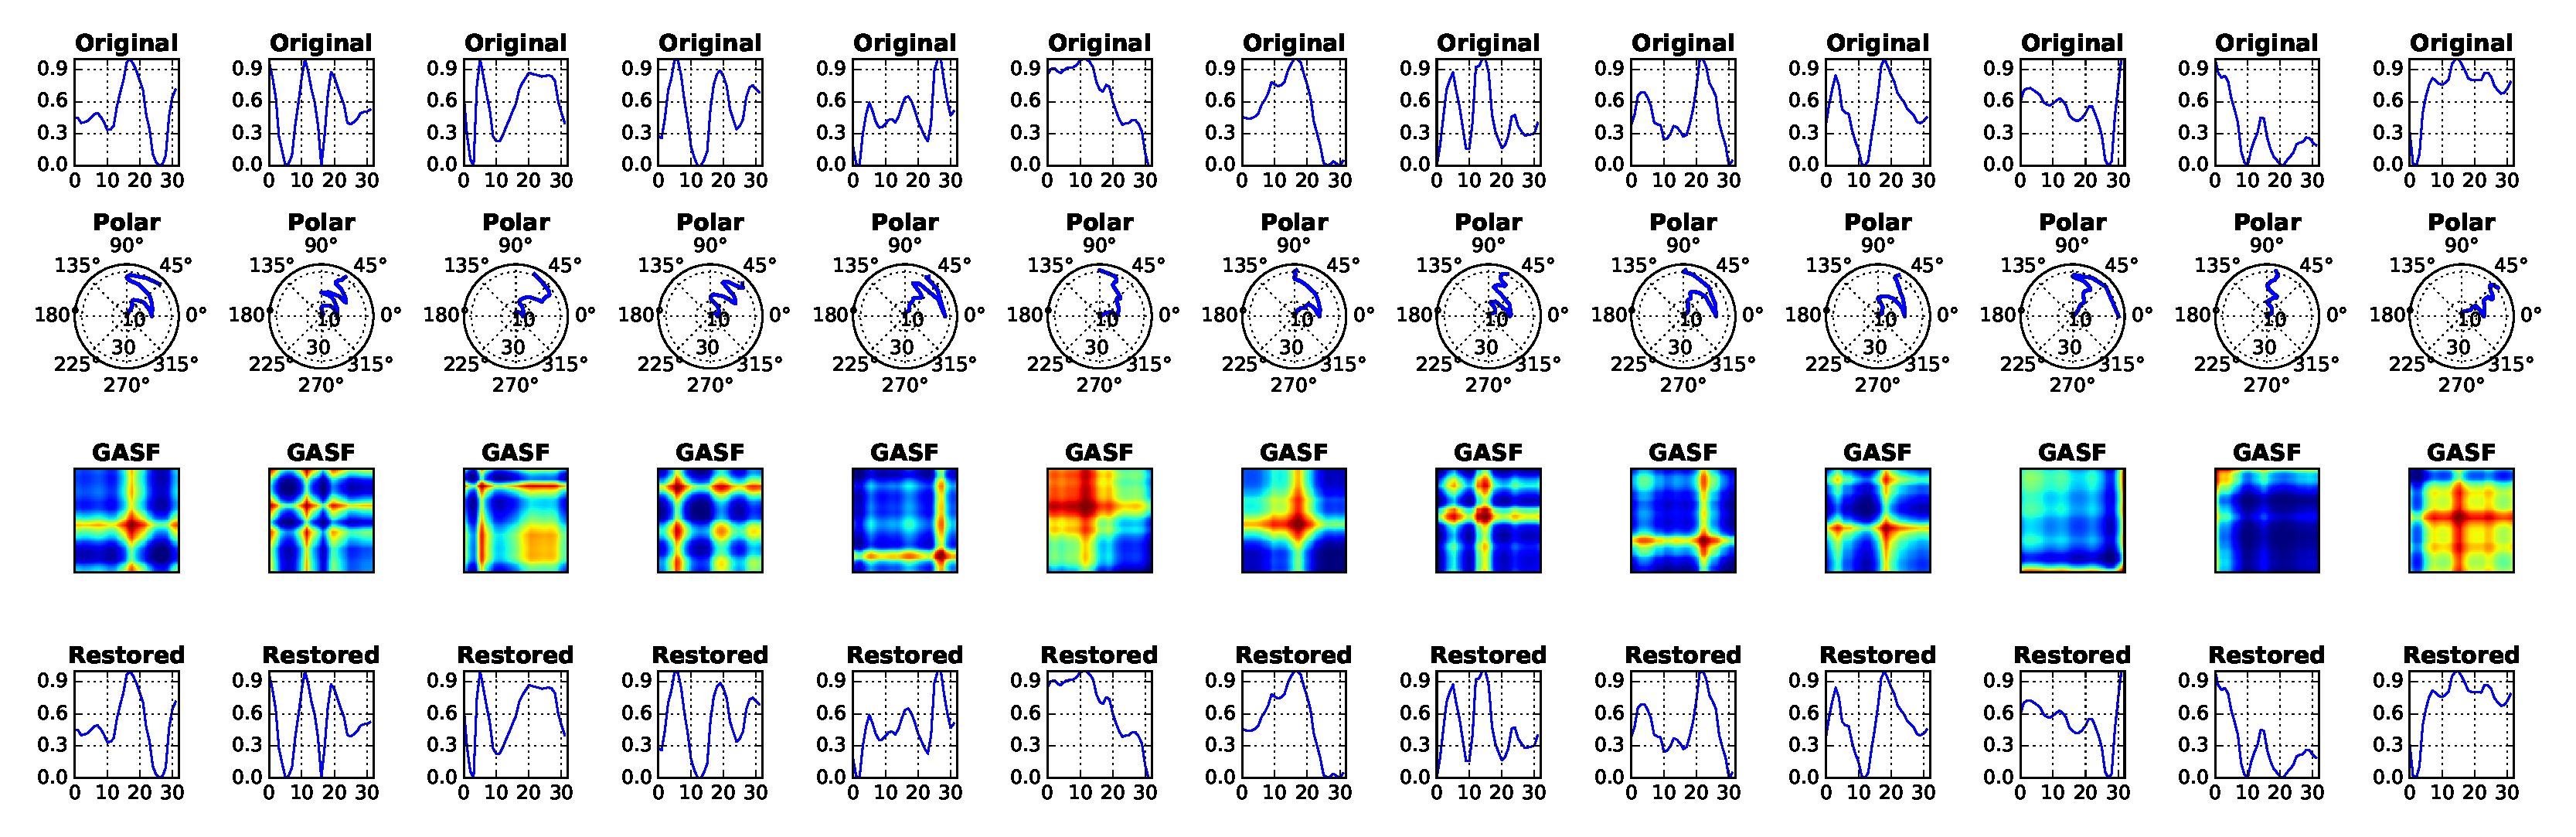
\includegraphics[width=.88\textwidth]{images/05-modeling/gasfpipeline.eps} 
 \caption{Conversion of time series into a Gramian Angular Summation Field (GASF) image and then back into its original space.}
 \label{figure:gasf_example}
\end{figure}

\subsubsection{Latent Dirichlet Allocation}
LDA is one of the most simple and influential topic models. {A topic model is a formal statistical relationship between a group of observed and latent (unknown) random variables, which specifies a probabilistic procedure to generate topics. The latter, in turn, is defined as a probability distribution over a collection of words}~\cite{reed_latent_2012}.

The graphical model shown in Figure~\ref{fig:graphical-model} presents the structure of the \gls{lda} model~\cite{blei_latent_2003}. Here, as in~\cite{smith_mining_2016}, the \textit{K}-th probability distribution over input words $\beta$ (called topics) is representative of the $K$ groups (types) of player motion styles in which we are interested. In turn, each document $d$ corresponds to a {game play} session for the game. We had to deal with the deterioration of model accuracy when considering the whole game section as a single document. Our solution for the problem was to segment each game section into subsets based on duration in seconds. %ANDY I cannot understand why couldn't be partitioned in subsets corresponding to the motion primitive, which already solved the problem. I'm losing my mind.
This approach raises several issues that are going to be properly addressed in a future work, but still allow one to obtain interesting~results. %ANDY This cannot be left like this. It is too open and undefined.

%\begin{figure}[H]
  \centering
  \begin{tikzpicture}
    [
      observed/.style={minimum size=15pt,circle,draw=blue!50,fill=blue!20},
      unobserved/.style={minimum size=15pt,circle,draw},
      hyper/.style={minimum size=1pt,circle,fill=black},
      post/.style={->,>=stealth',semithick},
    ]

    \node (w-j) [observed] at (0,0) {$w_{d,n}$};
    \node (z-j) [unobserved] at (-1.5,0) {$z_{d,n}$};
    \node (z-prior) [unobserved] at (-3,0) {$\theta_d$};
    \node (z-hyper) [label=above:$\alpha$] at (-4.5,0) {};
    \node (w-hyper) [unobserved] at (2,0) {$\beta_k$};
    \filldraw [black] (-4.5,0) circle (3pt);
    
    \node (eta-hyper) [label=above:$\eta$] at (3.5,0) {};
    \filldraw [black] (3.5, 0) circle (3pt);
    
    \path
    (z-j) edge [post] (w-j)
    
    (z-hyper) edge [post] (z-prior)
    (z-prior) edge [post] (z-j)

    (w-hyper) edge [post] (w-j)
    (eta-hyper) edge [post] (w-hyper)
    ;

    \node [draw,fit=(w-j) (z-prior), inner sep=14pt] (plate-context) {};
    \node [above right] at (plate-context.south west) {$D$};
    \node [draw,fit=(w-j) (z-j), inner sep=10pt] (plate-token) {};
    \node [above right] at (plate-token.south west) {$N$};
    \node [draw,fit=(w-hyper), inner sep=10pt] (plate-topic) {};
    \node [above right] at (plate-topic.south west) {$K$};
  \end{tikzpicture}
  \caption{LDA model diagram~\cite{blei_latent_2003}. Each word $w_{d,n}$ corresponds to a window of data from the accelerometer attached to the player during gameplay. In turn, a gameplay is interpreted as a document d (set of player generated words). $z_{d,n}$, represents the type (topic) assignment for a given word $w_{d,n}$ and $\theta_{d}$ is the mixture proportions representing the game session. In this work we are interested in representing the player game session by $\theta_{d}$.}
  \label{fig:graphical-model}
\end{figure}
%ANDY All the terms have to be defined. What is d? What are mixture proportions? What is D?
In these terms, a document may present multiple types $\beta_{k}$ with mixture proportions $\theta_{d}$ The mixture of proportions defines a player at each instant of time. The choice of the $N_{D}$ words comes from $\overline{\beta}_{d}$, which acts as the weighted average of the game play types for a given document. This average is defined as follows~\cite{blei_latent_2003,smith_mining_2016}:

\begin{equation}
\overline{\beta}_{d} = \sum_{n=1}^{K} \theta_{d}(k) \cdot \beta_{k}
\end{equation}

The \textit{n}-th word $w_{d,n}$ of document \textit{d} is, in our case, the GASF encoding obtained, as we will explain later. $z_{d,n} \in \{1:K\}$ refers to the random type from which a word is drawn. Following the standard \gls{lda} model, $\alpha$ and $\eta$ are hyperparameters that control the sparsity in the mixture proportions and word distributions~\cite{smith_mining_2016}.

\subsubsection{Autoencoder}\label{section:autoencoder}

In many problems, we may have to deal with highly dimensional data that represent the situation of the world as captured by the sensors. Given that the raw data dimensionality could be practically intractable, the common procedure in these cases is to reduce the dimensionality possibly keeping only the important features of the input data.

In image processing, for instance, understanding which pieces of an image represent a significant aspect for the task ahead is not a trivial issue. Significance may be related to specific parts of the image and may depend on many aspects. A common technique to face this issue is {autoencoder}.
Autoencoder is an unsupervised learning technique that learns a representation of the input data, usually derived by means of non-linear transformations of the input~\cite{goodfellow_deep_2016}.
A typical implementation of autoencoder consists of a feedforward neural network that first encodes the input into a code, the representation, and then reconstructs the input from it by means of a decoder (see Figure~\ref{fig:autoencoder_architecture}).

\begin{figure}[H]
\centering
\includegraphics[width=.9\columnwidth]{images/05-modeling/autoencoder_architecture}
\caption[Autoencoder general architecture]{General architecture of an autoencoder; the input layer is processed by an encoder that transforms it. The derived representation is then decoded by a decoder that yields a reconstruction.}
\label{fig:autoencoder_architecture}
\end{figure}

In general, autoencoders are good at capturing the structure of the input and tend to represent it well~\cite{goodfellow_deep_2016}. We can represent an autoencoder as a neural network that tries to copy its input to its output. We can represent its general architecture with the following terminology:
\begin{itemize}[leftmargin=*,labelsep=5.8mm]
	\item the input $x$,
  \item the {encoder function}, $f(x)$, composed of some hidden layers,
  \item the {code}, or internal representation, of the input $h$,
  \item the {decoder function}, $g(x)$, composed of other hidden layers,
  \item the reconstruction obtained from the decoder, $r$.
\end{itemize}

A {loss function}, $L(x, r)$, should also be defined to evaluate how close the reconstruction is with respect to the input.
A simple loss function is shown as Equation \eqref{eq:loss_autoencoder}.

\begin{equation} \label{eq:loss_autoencoder}
L(x,r) = \sum_{i} (x_i - r_i)^2
\end{equation}

However, if we do not impose any restriction, the transformation it learns would be an identity, since this would perfectly reconstruct the input. To prevent this transformation, two approaches have been devised~\cite{goodfellow_deep_2016}.
The first, called {undercomplete autoencoder}, adopts a representation smaller than the input (see Figure \ref{fig:under_over_autoencoder}a),
while the latter, {overcomplete autoencoder}, uses a representation with a dimension larger than the input (see Figure \ref{fig:under_over_autoencoder}b).
Although increasing the representation size is counterintuitive in order to sparsely represent the input, this technique has proven its effectiveness.

\begin{figure}[H]
\centering
\begin{subfigure}[H]{0.3\textwidth}
\centering
\includegraphics[width=0.9\textwidth]{images/05-modeling/undercomplete_autoencoder}
\caption{}
\label{figure:undercomplete}
\end{subfigure}
\begin{subfigure}[H]{0.3\textwidth}
\centering
\includegraphics[width=0.9\textwidth]{images/05-modeling/overcomplete_autoencoder}
\caption{}
\label{figure:overcomplete}
\end{subfigure}  \vspace{-6pt}
\caption{(\textbf{a}) Representation of an undercomplete autoencoder, where the representation has a lower dimension with respect to the input. (\textbf{b}) Representation of an overcomplete autoencoder, which uses a larger space to represent the input.}
\label{fig:under_over_autoencoder}
\end{figure}

The undercomplete autoencoder is the oldest and best known architecture for the autoencoder and also the one we use in our work. The code the autoencoder derives is smaller than the input: it learns how to combine the input so that the relevant information is retained in a lower dimensional space. The combination is often non-linear due to a non-linear activation function of the neurons. On~the other hand, the decoder function learns how to unroll such compressed code in order to obtain an extended representation. This architecture could be trained using the classic back-propagation approach, although different methods are available~\cite{goodfellow_deep_2016}.

The overcomplete autoencoder, instead, increases the dimension of the representation; however, as already mentioned, the model could easily learn the identity transformation. In order to tackle this issue, the common approach is to apply a regularization term over the weights of the network. In general, a $l_1$ penalization is added to the loss function.
In this way, the representation will be sparse since some of the dimensions are set to zero.
However, this new architecture would be more complex to train since the model would be larger than the previous one, although still providing a sparse representation.
Despite its sparsity, this architecture is able to extract more information from the input, and it is often used to capture also the input distribution and not just the structure of $x$. It is not possible to estimate such a distribution with an undercomplete autoencoder since such a task would require a higher representation capacity.

In this work, we adopt an undercomplete autoencoder, since our goal is to represent an image in a lower dimensional space. 
Our architecture has multiple layers: the first layer takes only the input, while the following ones decrease in size with the power of two.
We represent the input with a code having 64 dimensions; thus, from an input of 1024 features, we derive a representation of 64 components using an autoencoder.

The reconstruction of the input by the decoder function has a very low loss, below 0.05$\%$. The~layers obtained by the encoder are often difficult to understand by people; for instance, in Figure~\ref{fig:levels_autoencoder}a--c, we can observe the first layer, and we cannot derive any structure or meaning from it.
However, looking at deeper levels, the layers show a clear structure; in Figure~\ref{fig:levels_autoencoder}g--i, we can observe that the filters are extracting horizontal and vertical patterns. Indeed, most of the original images show a cross pattern, or multiple crosses; therefore, this representation seems to be able to represent the input data with a lower dimension.

\begin{figure}[H]
\centering
\begin{tabular}{ccc}
\includegraphics[width=0.2\columnwidth]{images/05-modeling/autoencoder_levels/autoencoders_2_0} &
\includegraphics[width=0.2\columnwidth]{images/05-modeling/autoencoder_levels/autoencoders_2_1} &
\includegraphics[width=0.2\columnwidth]{images/05-modeling/autoencoder_levels/autoencoders_2_2} \\
(\textbf{a}) & (\textbf{b}) & (\textbf{c}) \\
\includegraphics[width=0.2\columnwidth]{images/05-modeling/autoencoder_levels/autoencoders_4_0} &
\includegraphics[width=0.2\columnwidth]{images/05-modeling/autoencoder_levels/autoencoders_4_1} &
\includegraphics[width=0.2\columnwidth]{images/05-modeling/autoencoder_levels/autoencoders_4_2} \\
(\textbf{d}) & (\textbf{e}) & (\textbf{f}) \\
\includegraphics[width=0.2\columnwidth]{images/05-modeling/autoencoder_levels/autoencoders_7_0} &
\includegraphics[width=0.2\columnwidth]{images/05-modeling/autoencoder_levels/autoencoders_7_1} &
\includegraphics[width=0.2\columnwidth]{images/05-modeling/autoencoder_levels/autoencoders_7_2} \\
(\textbf{g}) & (\textbf{h}) & (\textbf{i}) \\
\end{tabular}
\caption{Example layers from the trained autoencoder. (\textbf{a}--\textbf{c}) represent the information extracted by the first layer of the autoencoder. It is hard to grasp the meaning of the representation derived. Going deeper, in (\textbf{d}--\textbf{f}), the representation seems to become more clear and with a structure. Indeed going directly to the obtained code, in (\textbf{g}--\textbf{i}), we can see a more accentuate structure composed mainly of horizontal or vertical lines.}
\label{fig:levels_autoencoder}
\end{figure}

\subsection{Problem Statement} %ANDY this section seems fundational, an probably should stay at the beginning ofthe chapter. Frmulating a problem is typically done before than proposing solutions.
This section formulates the problem of modeling the player as a probabilistic mixture of player styles derived from data. There are at least three basic dimensions (or problems) of interest that must be considered when building a model of this kind for \gls{pirg}s. Such dimensions are related to the specific capabilities of a mobile robot to achieve a suitable in-game performance. We delineate such dimensions as follows:

\begin{itemize}[leftmargin=*,labelsep=5.8mm]
\item {Dimension \#1: Fundamental robot behavior}, which concerns the fundamental aspects of the robot locomotion, timing of actions, localization and other abilities to keep it alive and well-functioning during the game play.
\item {Dimension \#2: In-game competitive capabilities}, which are more related to the intelligent selection of actions aimed at achieving in-game goals. In other words, this dimension captures the intricacies of planning and rational behavior, using solutions developed for Dimension \#1.
\item {Dimension \#3: Adaptive power}, which is a higher level dimension concerned with how and when during the game to adjust the robot performance to match that of the current player.
\end{itemize}

Dimension \#1 concerns the setup of an appropriate robotic platform, including aspects like: electrical disturbances, power consumption, kinematic constraints, processing capabilities, sensing and safety. These are recurrent issues that must be appropriately dealt with. 

Dimension \#2 encompasses the problem of finding a plan or strategy to achieve the robot goals. This is the problem most related to the competitive behavior the robot can impose on the human player, since action selection is driven by the tendency to maximize the robot's own pay-off. After all, the robot has to give the idea that it is at best trying to beat/help its opponent(s)/companion(s).

Dimension \#3, based on \#1 and \#2, defines constraints on the robot behavior such that the action selection is not longer just governed by the tendency to be competitive/helpful, but is also driven by the compelling necessity to support the player interaction, in real time, as robustly as possible.

One can see that the present work as a step towards advancements in Dimension \#3.
%ANDY All this would be nice in the introduction of this thesis, and could drive the presentation, showing as you have faced all these aspects, producing innovative results in some of them. Player modeling is missing here, and could go in \#3, being \#1 dedicated to development of a fully funcyional body, \#2 to the ability to play, and act according the rules, including the ability to aim at winning, descpite the player, while \#3 considers also the player, models it, and try to optimize entertainment more than performance in the game, eventually reducing the robot's abilities. Your main contribution is, of course on \#3, but you had to face also the other two, and, actually, you have to describe them UP to now you haeve described \#1 and part of \#3. #2 is missing at this point, but surely will be in the following.

Here, we exploit data coming from a single accelerometer placed on the human player's body; thus, player movement is our primary source of information for describing the playing style and engagement. 
%ANDY However you have also mentioned IC, and other image-based features. You should take a definite line, putting in evidence clearly what you have explored and then left and whatis teh content of the final proposal, which, BTW, seemed to be based on lasers only, losing the richness provided by the other data sources (accelerometer and Kinect) and the possibility to explore and exploit data fusion.

The basic assumption is that a highly active player would naturally express his/her status by a very turbulent motion signal that is compatible with strong in-game activity. Consider, for instance, the difference in signal shapes reported in Figure~\ref{figure:acc_signal_shape}.

Following this line of reasoning, we also assume players do not fake their engagement by unnecessarily performing strong activities, like running, when they are actually not engaged in the game or feel bored by the robot behavior. Therefore, we assume that a highly motivated player would act more intensively and frequently than a non-motivated one, thus showing a more turbulent acceleration signal profile.

In situations like \gls{pirg}, movement information is useful and should not be disregarded. Furthermore, a model that is able to extract a description of the player's movement profile for the purpose of robot behavior adaptation would generate interesting dynamics able to hide existing platform limitations (kinematics constraints, tracking problems, etc.) and boost game experience.

One important aspect not considered yet by our assumptions is the role of skill level. For example, a highly skilled player could try to minimize his/her energy expenditure by performing precise movements towards winning the game and in theory could perfectly show a low-movement profile. Moreover, these assumptions cannot directly measure player engagement in the game, given that it is also possible for a player to move not too much, but, at the same time, be highly engaged. 

In summary, we are interested in investigating time series data, especially acceleration patterns as proxy and/or engagement cues (given the mentioned assumptions) towards the creation of auto-adjusting robotic companions or opponents.

%ANDY The last 4 paragraphs present nice ideas, but they seem unrelated to each other, just put here as they come to the mind. These considerations are good for the introduction, and the conclusion chapters, and should be integrated with their developments throughout the text.




\begin{figure}[H]
\centering
\begin{subfigure}[H]{\textwidth}
\centering
\includegraphics[width=0.2\textwidth]{images/05-modeling/enricorun.png} 
\includegraphics[width=0.6\textwidth]{images/05-modeling/running_sig_profile.eps} 
\caption{}
\end{subfigure}

\begin{subfigure}[H]{\textwidth}
\centering
\includegraphics[width=0.2\textwidth]{images/05-modeling/enricostill.png}
\includegraphics[width=0.6\textwidth]{images/05-modeling/standing_sig_profile.eps} 
\caption{}
\end{subfigure} \vspace{-6pt}
\caption{Three-axis accelerometer signal during game play. (\textbf{a}) A running player. (\textbf{b}) A player standing still. Notice that signal shape and amplitude are very characteristic for the respective activity.}
\label{figure:acc_signal_shape}
\end{figure} \unskip

\begin{figure}[H]
\centering
\begin{subfigure}[H]{\textwidth}
\centering
\includegraphics[width=0.6\textwidth]{images/05-modeling/example_signal.eps}
\label{figure:accelerometer_signal}
\caption{}
\end{subfigure} \vspace{-6pt}

\begin{subfigure}[H]{\textwidth}
\centering
\includegraphics[width=0.45\textwidth]{images/05-modeling/example_gafs_seg.eps}
\caption{}
\end{subfigure} \vspace{-6pt}
\caption{Example of the conversion of a time series into GASF images. (\textbf{a}) Three-axis accelerometer data (48.8 Hz) of about 30 seconds of real game play. (\textbf{b}) Thirty five GASF segments of a linear combination of the multidimensional time series. Each window comprises 0.65 seconds with 32 samples.}
\label{figure:acc_signal_gasfs}
\end{figure}


\subsection{Activity modeling}
This section describes our approach to model the activity of the player, while emphasizing the differences and similarities with respect to existing methods. We take inspiration from approaches like~\cite{smith_mining_2016, wang_encoding_2015, wang_imaging_2015} and aim at modeling game sessions as ``documents'', where player's acceleration data are considered as ``words''. We use LDA~\cite{blei_latent_2003} to categorize the player's motion profile as a composition or mixture of game play motion types, the latter being analogous to the ``topics'' in the general application of \gls{lda} for document modeling.

Differently from~\cite{smith_mining_2016}, our input word atoms are not discrete. Instead, they are continuous (acceleration data) and also are not attached to any explicit meaning. Take, for instance, the natural interpretability of joystick input signals like ``left'' and ``right'', which convey their respective meaning when controlling a game character, and compare it with an acceleration signal that carries no obvious absolute meaning.

The method adopted for selecting the input words is based on sliding windows (just as in~\cite{smith_mining_2016}), without overlap. %ANDY This choice should be justified, even more since few sections above you discussed the sliding window concept and adopted a different criterion.

Considering each game session as a document, the windowed segments play the role of words. Since the space is continuous, a procedure of discretization and dictionary learning for \gls{lda} had to be performed. For this, we clustered the segments and used the so-obtained cluster centroids as dictionary words.

We have used GASF images instead of GADF because the mapping functions of the rescaled time series in $[\,0,1]\,$ are bijections, which allows for precise reconstruction of the original time series~\cite{wang_imaging_2015}. The reconstruction takes advantage of the the main diagonal of GASF, i.e., $\{G_{ii}\} = \{\cos{2\phi_{i}}\}$, and is performed as reported in Equation~(\ref{equation:reconstruction})~\cite{wang_imaging_2015}: 
%%Please note that the citation of figures should be in numerical order, figure 8 appeared before figure 7, please revise.
\begin{equation}\label{equation:reconstruction}
\cos(\phi)=\sqrt{\frac{G_{ii}+1}{2}} \qquad \phi \in [\,0,\frac{\pi}{2}]\,
\end{equation}

An example of signal decomposition into GASF images is shown in Figure~\ref{figure:acc_signal_gasfs}. Given recent advances in deep learning and pattern recognition for images, we take the route of~\cite{wang_encoding_2015} and exploit the applicability of autoencoders for extracting unsupervised features from GASF images (see Section~\ref{section:autoencoder}). This is relevant since the process of feature engineering is time-consuming and laborious. Moreover, unsupervised feature extraction from such methods has been proven to work well~\cite{wang_imaging_2015, wang_time_2016}.
Sparse encoding via linear-algebra methods for dictionary learning is also a possibility. However, in our experiments, it turned out to be not as efficient as autoencoders. We present details of our experimental activity in the next section. Our methodology is summarized in {Figure~\ref{diagram:methodology}.

%\begin{figure}[H]
%	\centering
%\begin{tikzpicture}[auto]
%	\tikzstyle{b} = [rectangle, draw, fill=blue!20, node distance=0.5cm, text width=4em, text centered, rounded corners, minimum height=5em, thick]
% \tikzstyle{c} = [rectangle, draw, inner sep=0.2cm, dashed]
% \tikzstyle{l} = [draw, -latex',thick]
%
%  \node [b] (time series) {Game time series};
%  \node [b, right=of time series] (segments) {Segments};
%  \node [b, right=of segments] (gasfs) {GASFs};
%	\node [b, right=of gasfs] (features) {GASFs features};
%  \node [b, right=of features] (dict) {Dict. Learning};
%  \node [b, right=of dict] (lda) {LDA};
%
%  \path [l] (time series) -- (segments);
%  \path [l] (segments) -- (gasfs);
%  \path [l] (gasfs) -- (features);
%  \path [l] (features) -- (dict);
%  \path [l] (dict) -- (lda);
%\end{tikzpicture}
%\caption{The general diagram for our methodology. At first, game time series are extracted, which are then segmented into windows (sliding windows method). Such segments are then turned into GASF images, whose representations are obtained using the autoencoder. Since the basic \gls{lda} method works with a multinomial distribution at the topics, we define a dictionary of visual words before feeding each GASF feature document representation to it.}
%\label{diagram:methodology}
%\end{figure}

\subsection{Experimental Results}
In this section, the exploration of an incomplete representation of the GASF images using a simple autoencoder architecture is firstly reported, then we discuss how we transform the extracted features into input words for the \gls{lda} model. Finally, we show the results when confronting the model output with human judgment. All experimental code used is available at the link in supplementary materials. %ANDY Check that this is actually available and report the link here

\subsubsection{Feature Extraction}

The first question we need to answer concerns the size of the sliding window. This parameter regards the definition of the GASF images used as building blocks for the dictionary learning. The~window size should be large enough to capture motion patterns relevant for the player characterization, but not so large to confound their interpretation. We tried different window sizes, and in the end, we followed~\cite{oliveira_activity_2017} and decided to consider half a second of data per window without overlap, which allows for a quite fine-grained data representation.

We applied no preprocessing to the signal, since we were interested in observing how an autoencoder would perform using the unfiltered input. The expectation was that it would naturally compensate for the differences in the images, decisively choosing to capture important features (the main signal characteristic) and disregarding non-representative ones (the small associated noise). We defined an architecture composed by dropout and dense layers where only hyperbolic tangent activation functions where used, except in the last layer, where a linear activation function was used instead. The best performing architecture was composed by the following layers: dropout (0.1 drop fraction), dense (size = 256), dropout (0.2) and dense (size = 64). The same layers (in reversed order) were used for the decoder part.

A window of half a second corresponds to 32 samples given our accelerometer average frequency of 48.8 Hz. As a consequence, we obtain GASF images (without using PAA) with a total of 1024 pixels. Using the autoencoder, we manage to reduce the representation down to a 64-dimensional input, resulting in the reconstruction presented in Figure~\ref{figure:reconstruction}. The choice of a 64-dimensional representation is empirical, meaning that we were in principle searching for an incomplete representation of the data and, upon testing with different configurations, we have chosen the one with the lowest reconstruction error. As it turned out, a 64-dimensional vector representation was the best result, given our dataset. 

\begin{figure}[H]
	\centering
	\includegraphics[width=.9\textwidth]{images/05-modeling/reconstructions.eps}
	\caption{Autoencoder reconstruction for five input segments corresponding to half a second of data (linear combination of the acceleration axis). ({Top line}) Input GASF images. ({Second line}) Original time series for each GASF input. ({Third line}) The autoencoder reconstruction for the input images. ({Forth line}) Time series from the reconstructed GASF images.}
  \label{figure:reconstruction}
\end{figure}

It is possible to notice from the reconstruction result that, despite such a large compression (from 1024 to only 64 values), the input image relevant structure is captured. This can also be seen in the reconstructed time series. A closer look reveals that the autoencoder practically smoothed the time series while preserving the overall shape, this being a nice property that can help to prevent overfitting.

From Figure~\ref{figure:reconstruction}, we can also see that the obtained time series reconstruction presents some holes. This seems to be caused by the information loss in the reconstruction and demands further investigation. However, in our experimentation, it did not seem to affect the learning performance. 

\subsubsection{Dictionary Learning and Input Word Definition}
Latent Dirichlet allocation works by considering the relationship among word tokens with respect to a collection of documents. Therefore, in order to use the method, we needed to come up with a way to encode the taxonomy of GASF images into a discrete set of fixed tokens describing the motion primitives appearing in each game session. We opted to follow~\cite{prince_computer_2012} and encode the features extracted from the GASF using the autoencoders as visual words, composing the game session document.

After getting the 64-dimensional vector representation for each GASF image (see Section~\ref{section:autoencoder}), we cluster them into $V$ groups using the K-means algorithm. In this way, we define a dictionary of size $V$, with each word corresponding to a cluster centroid. Each game session is then translated into a collection of $V$ possible clusters, which can then be fed into the \gls{lda} algorithm.

From text mining and information retrieval, we know that having documents with different sizes can rise critical issues. This is because given the bag of words representation used in \gls{lda}, a small document may be included as a subset in a larger one. Additionally, it might be a problem to evaluate longer documents in our scenario, since, at least from a human perspective, it is not simple to define the overall behavior. %ANDY I'm missing this

In text mining, this issue is handled by imposing a weight based on the length of the document; in our case, instead, we decided to split each session into smaller segments of 15 s each. In this setting, the evaluation is more consistent, and it is possible that the behavior of a player will be maintained within segments. We decided this length for each document both for convenience with respect to the window length and from the assumption that in each fraction of 15 s, the player can show a consistent behavior, which can be somehow easily identifiable. In the next section, we present the results achieved with the approach we just presented.

\subsection{Validation}

Our ultimate objective is to represent the player motion style by a mixture of topic proportions following the \gls{lda} framework. Unfortunately, the method by itself demands the programmer to initialize the desired number of topics. Thus, we had to perform a search for the optimal value given our dataset.

By performing grid search, we selected a range of values for the two main hyperparameters, namely dictionary size, for the input word definition, and number of topics. We would like to keep the number of topics low, preferably less than 10, since by observing our dataset, it is not possible to distinguish many groups of different motion styles; this suggests that a coarse-grained definition would be better. Choosing the number of topics to be at most 10, as in~\cite{smith_mining_2016}, the evaluation of the uncovered topics remains manageable, while maintaining a certain degree of freedom for the existing motion diversity.

The distribution of cluster centroids (words) given topics (our player motion types) is shown in Figure~\ref{overallgame}.
Each line represents a topic, while each column represents a word. As one can see, there are no topics represented by the same distribution over the same word. Figure \ref{overallgame} shows how much each word is important for the specific topic.

\begin{figure}[H]
	\centering
	\includegraphics[width=\textwidth]{images/05-modeling/lda_heatmap.eps}
	\caption{Schematic representation of the game: each line represents a topic, while each column represents a word that is representative of the specific topic.}
  \label{overallgame}
\end{figure}

In order to validate the discovered topics, we use human judgment. We invited volunteers to watch a set of pairs of recorded game segments (15 s each) and point out the similarities between players in their motivation as perceived by their motion. Subjects had to judge how similar, on a scale from 0--5, the movements of two players were. With this, we generated a similarity matrix to be used as the ground truth and main guide for deciding which hyper-parameter value to use and to check whether the proposed method could achieve reasonable results.

The similarity matrix was composed of $406$ independent evaluations from six different human subjects. The generated evaluation matrix was then compared with a cosine similarity matrix generated after training the \gls{lda} in our dataset. The similarity, in this case, is based on the mixture proportions among the discovered topics. 

We used this information to define the number of topics and the number of words. The best set of parameters is the one that presents a higher similarity compared to the one expressing human judgment, thus the smallest Mean Squared Error (MSE). The graph in Figure~\ref{hyperparameter_results} shows the results obtained varying the size of the dictionary (number of cluster centroids) and the number or topics. From it, we have decided to pick 100 as the number of visual words and 10 for the topics present in our dataset.

\begin{figure}[H]
	\centering
	\includegraphics[scale=0.6]{images/05-modeling/mse_dictsize-50_100_10.png}
	\caption{The figure shows the hyperparameter tuning results. The Mean Squared Error (MSE) is estimated with respect to the similarity expressed in the matrix containing the human judgment. The different lines represent the MSE obtained for different dictionary sizes and number of topics.}
  \label{hyperparameter_results}
\end{figure}

The observed similarity results were verified by visual inspection of video logs from estimated similar players; that is, by checking how reported mixture proportions actually look similar in video. However, we state that much work should still be performed towards easily and reliably assessing model correctness and selection. This also relates to the possibility of confidently giving names to discovered motion types, very much in the way as is done in classic \gls{lda} for text categorization.

Another aspect that demands further investigation is how to avoid the decrease in accuracy when considering variable-sized game sessions. As mentioned before, game sessions with different sizes may artificially increase similarity in case one is a subset of another. The solution to this problem provides only a baseline, and much more sophisticated approaches to the problem should be~devised.

We believe that a potential way for improvements in interpretability and accuracy is that of removing the vector quantization in defining each topic. It would be interesting to remain in the continuous domain defined by our input data representation (GASF features), instead of relying on a fixed predefined vocabulary set used for training the \gls{lda}. Such vectorization is known to lead to information loss~\cite{hu_latent_2012}. To avoid such an issue, one possibility may be replacing the topic multinomial distribution by a mixture of Gaussians~\cite{hu_latent_2012}.

\subsection{Discussion}
In this work, we introduced an approach to identify the player motion styles from measurements obtained by the use of a single three-axial accelerometer sensor. Such a signal is then transformed using the Gramian angular field in an image that represents its content. The reason for such representation stems from recent publications aiming at using deep learning and state-of-the-art image processing techniques for achieving better classification results. Additionally, using the autoencoder for representing the obtained GASFs reduced the workload necessary for hand-crafting features, as often done when using machine learning classification/clustering methods with time series data.

By applying latent Dirichlet allocation to characterize the motion behavior of different players, we were interested in getting a description that would foster the development of self-adjusting \gls{pirg}s agents capable of improving/sustaining engagement. In this, we had shown that the model is able to capture the overall human judgment by matching reported similarities. 

This is the first work, to our knowledge, that tries to model the motion behavior of the player using this type of signal in conjunction with \gls{lda} in a robogame scenario. We have demonstrated that the proposed approach is able to cluster and represent different behaviors learned from data. We have evidence that our methodology can achieve better performance than that of relying solely on the measurements of the accelerometer as input for the dictionary learning step. We are still working to provide a fair comparison between the two approaches.%ANDY Another thing to do

As future work, we want to test our approach with a series of different input signals in order to assess its capability. One alternative could be the incorporation of proximity information in order to capture how proximity patterns relate to a player game play style. Moreover, we are interested in measuring the player's effort expenditure in terms of difficulty of motion given a difficult setting for the robot. 

In our method, we also wish to incorporate time dependency. We believe such information would help to describe variations in playing style during play, given the opportunity to detect change points in styles and favor game (robot behavior) personalization. This also may help to avoid the rubber-band effect, a system instability concern often present when designing auto-adjusting game systems.

Another means for improvements, and one that we are currently working on, is that of removing the vector quantization step necessary for the definition of the multinomial distribution of words that defines each topic. We believe that it would be interesting to remain in the continuous domain defined by our input data, instead of relying on a fixed predefined set of tokens, i.e., the vocabulary set used for training the \gls{lda}. Our current experimentation goes along the lines of testing how a Gaussian version of \gls{lda} would work in our domain and whether that could give better results. Additionally, comparing our results with a continuous version of \gls{lda} would help to answer questions regarding {stop word} filtering, such as: To what extent removing certain common segments would improve or worsen accuracy?

Finally, we are working to redesign the experiments in order to allow for collecting user survey data, which comprise a valuable resource regarding player style and engagement levels. This is all in order to increase our understanding of the obtained results. We plan to collect self-reported engagement levels when comparing with different robot behavior configuration while allowing for adaptation. Regarding such adaptation, we currently are investigating how to relate the robot game's difficult settings (such as velocity, tower LED control rules, among others) and the mixture proportion of motion types discovered by our reported method. One alternative is to design a utility function that would describe what is the pay-off in facing a certain player given a certain difficult setting, therefore turning the adaptation problem into a full on-line optimization procedure where we try to match player motion types with robot behavior implied by difficulty settings.

%ANDY Future work has to be cited, however, this is not a paper, but a PhD thesis. Future work related to other parts of the thesis (such as experiments on different behaviors) should take them into account, and experimens should (have) consider(ed) all the aspects to be investigated.
